\RequirePackage{luatex85}
\documentclass[tikz]{standalone}
\usepackage{tikz-feynman}

\begin{document}
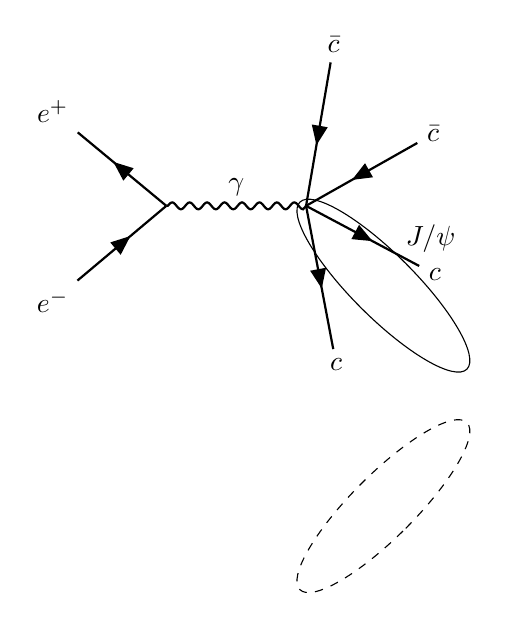
\begin{tikzpicture}
    \begin{feynman}
        \diagram [horizontal=EEG to GCC,large] {
            e [particle=\(e^-\)] -- [fermion] EEG -- [fermion] ebar [particle=\(e^+\)],
            EEG -- [photon, edge label=\(\gamma\)] GCC,
            c1bar [particle=\(\bar{c}\)] -- [fermion] GCC -- [fermion] c1 [particle=\(c\)],
            c2bar [particle=\(\bar{c}\)] -- [fermion] GCC -- [fermion] c2 [particle=\(c\)],
            c1bar -- [plain, opacity=0] -- c2,
            c2bar -- [plain, opacity=0] -- c1,
        };
    \end{feynman}

    \begin{scope}[shift={(4.2cm,0.2cm)}]
        \draw[rotate=45] (0,0) ellipse (0.4cm and 1.5cm);
        \node at (0.6cm,0.6cm) {\(J/\psi\)};
    \end{scope}

    \begin{scope}[shift={(4.2cm,-2.6cm)}]
        \draw[rotate=-45, dashed] (0,0) ellipse (0.4cm and 1.5cm);
    \end{scope}
\end{tikzpicture}
\end{document}
